% $Id: chapter3.tex 1790 2010-09-28 16:46:40Z jabriffa $

\chapter{Technical Review}

This chapter will go in depth about technical side of the project. It will start off with the dataset that being used. Then, it will discuss the resources that will be used and where the code and the models will be from. After then, will walk through each of the models that are implemented and the usage of libraries and methods.

\section{Dataset}
The dataset that is used to train and test is from \textit{"Emotion Dataset for Emotion Recognition Tasks"} \cite{Pandey_2021} from Kaggle which is based from \textit{"CARER: Contextualized Affect Representations for Emotion Recognition"} \cite{saravia-etal-2018-carer} paper. It is an English Twitter message dataset, and it has 6 labels: sadness (0), joy (1), love (2), anger (3), fear (4) and surprise (5). It is for single-label emotion classification task, and it is already separated into train, test and validation dataset. 

\textbf{An example of 'train' dataset:} 

\emph{"label": 0,}

\textit{"text": "im feeling quite sad and sorry for myself but ill snap out of it soon" }

\begin{figure}[h!]
    \centerline{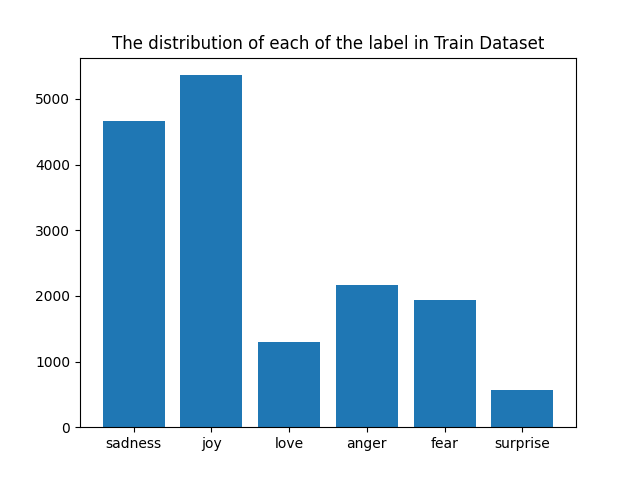
\includegraphics[scale=0.5]{Figures/dataset_distribution.png}}
    \caption{The graph for the distribution of each label in Train dataset}
    \label{fig:dataset}
\end{figure}

For the training dataset, the distribution of labels of the emotion data is not equal; "surprise" has the lowest distribution and "joy" has the highest. The distribution is displayed in Figure(\ref{fig:dataset}).



\section{Methods}

This section will dive deeper into each pre-trained model, and how it is implemented, what libraries have been used and why. The 4 pre-trained transformer models that are implemented for this research are as mentioned in literature review which are miniLM, Llama2, RoBERTa and GPT-2.

\begin{figure}[ht]
    \centerline{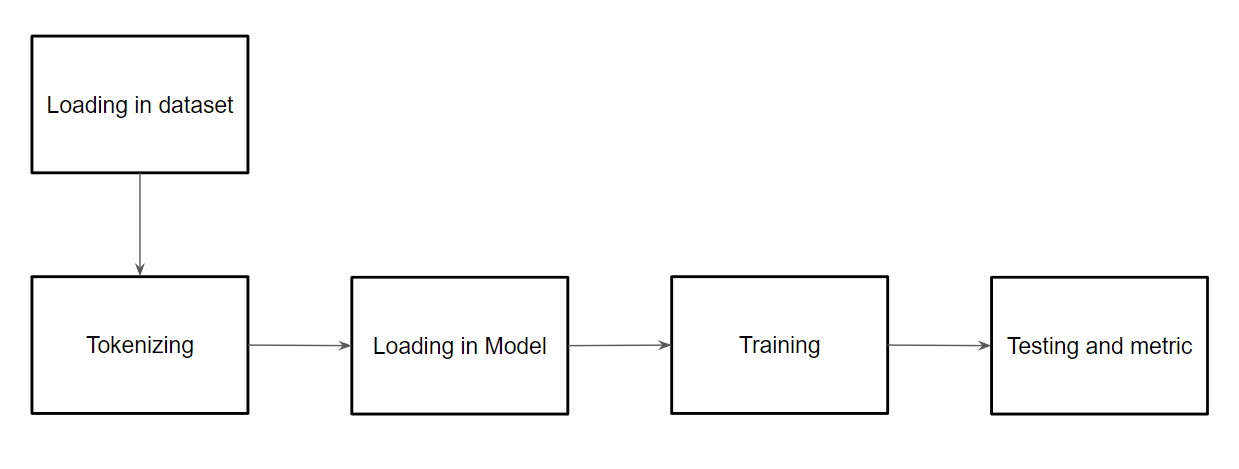
\includegraphics[scale=0.45]{Figures/problem_pipeline.png}}
    \caption{A pipeline of the overall flow of implementation}
    \label{fig:pipeline}
\end{figure}

The Figure[\ref{fig:pipeline}] shows the overall implementation of each model. The code for all the model will be followed roughly as the figure portrays and will be sectioned as such: Import libraries, Dataset, Model, Training and Testing/Evaluation. The implemented models will be run as Notebooks on either Google Colab or locally (in Vscode) depending on how big the model is.

The main benefit of using notebooks for the implementation is ability to break sections of code into blocks of code or 'cells' to make it easier to see and follow through. It also makes sectioned code easier to test and check for errors. For example, if the variables or code need to be checked to ensure their functionalities, or to check the features of datasets, cells can be added to verify and deleted after. Another benefit is that the cells can be 'markdown cells' which makes sectioning the code easier, can write titles and paragraphs overviewing each section, allowing anyone to understand the implementation quicker.

For the implementation of this study, all the pre-trained models used were taken from HuggingFace \cite{Hugging_Face}. HuggingFace is a substantial platform for an AI community. It's also accommodating for any new keen learner with their work through videos and documents. It also provides many tools such as different models, datasets, accessibilities to any Ai applications made by the community, documents for specific libraries and methods, solutions and finally an ability to communicate or ask about any Ai related queries with other members in the community.

\section{Main libraries}
The following are the libraries used throughout all the models that are implemented, and the brief descriptions of their use and what they provide:

\textbf{Torch:} an essential python library which allows machine learning algorithms to run faster than if they were written in normal python. It also supports 'Cuda' to run models on the GPU.

\textbf{Datasets:} a library that provides easy access for loading in datasets from huggingface as well as your own datasets.

\textbf{Transformers:} give an ability to load in all the transformer models, provide tools such as Trainer, TrainingArguments and so on and pipeline from the huggingface.

\textbf{Pandas:} used for reformatting and organizing the datasets without actual changes to the datasets.

\textbf{TQDM:} displays progress of the model training and testing.

\textbf{Numpy:} a python library that supports and operates on large multidimensional arrays and matrices along with variety of mathematical functions.

\section{Loading datasets}

By using \textbf{"Datasets"} library, \textit{load\_dataset, ClassLabel and Features} are imported. To load all the dataset from the folder, \emph{Load\_dataset} is used. 

However, the dataset come without the \emph{ClassLabel}. It is useful to have in the dataset's features as the model can relate the label indices with the \emph{ClassLabel}. Without it, the labels are just numbers and there are no correlation with the emotions or have any context for them. Therefore, the function for adding in the \emph{ClassLabel} is implemented, and the code and its output can be seen in the listing(\ref{lst:classlabel}). 
\bigskip

\lstset{style=mystyle}
\begin{lstlisting}[language=Python, caption=The code for adding \emph{ClassLabel} and its results, label=lst:classlabel]
    df = my_dataset["train"].to_pandas()
    labels = ['sadness','joy','love','anger', 'fear', 'surprise']
    ClassLabels = ClassLabel(num_classes=len(labels), names=labels)
    
    # Mapping Labels to IDs
    def map_label2id(example):
        example['label'] = ClassLabels.str2int(example['label'])
        return example
    
    my_dataset= my_dataset.map(map_label2id, batched=True)
    
    # Casting label column to ClassLabel Object
    my_dataset = my_dataset.cast_column('label', ClassLabels)


Output: {'text': Value(dtype='string', id=None), 'label': ClassLabel(names=['sadness', 'joy', 'love', 'anger', 'fear', 'surprise'], id=None)}
\end{lstlisting}

\section{Prompt and Prompt Engineering}

A prompt is needed for training and testing the dataset as Llama2 model uses prompt engineering. Prompt engineering is a process of optimising prompts, queries and instructions for machine learning or AI models to output desirable results or predictions\cite{McKinsey_2024}. Which means that a sentence such as "i didnt feel humiliated" is not a sufficient prompt for the model to train or test with. Thus, an additional text is added before every sample text in all the dataset. The text prompt added is \textit{"Analyze the emotion of the texts in the square brackets, determine if it is sadness, joy, love, anger, fear, surprise, and return the answer as the corresponding sentiment label "sadness","joy","love","anger", "fear", "surprise""}. The code for this can be seen below in the listing(\ref{lst:prompt_adding}).

\begin{lstlisting}[language=Python, caption=The code for adding an additional prompt before the sentences, label=lst:prompt_adding]
def generate_prompt(data_point):
    return f"""
            Analyze the emotion of the texts in the square brackets,
            determine if it is sadness, joy, love, anger, fear, surprise, and return the answer as
            the corresponding sentiment label "sadness","joy","love","anger", "fear", "surprise".

            [{data_point["text"]}] = {data_point["label"]}
            """.strip()

def generate_test_prompt(data_point):
    return f"""
            Analyze the emotion of the texts in the square brackets,
            determine if it is sadness, joy, love, anger, fear, surprise, and return the answer as
            the corresponding sentiment label 'sadness','joy','love','anger', 'fear', 'surprise'.

            [{data_point["text"]}] = """.strip()

X_train = pd.DataFrame(X_train.apply(generate_prompt, axis=1),
                       columns=["text"])
X_valid = pd.DataFrame(X_valid.apply(generate_prompt, axis=1),
                      columns=["text"])

y_true = X_test.label
X_test = pd.DataFrame(X_test.apply(generate_test_prompt, axis=1), columns=["text"])
\end{lstlisting}


\section{Preprocessing}
Preprocessing the data before the diving into training and testing the models is necessity as stop words, upper or lowercase, punctuations and so on can hinder the model to learn or understand the input data. Fortunately, the dataset has already been preprocessed by removing punctuations, lowercasing all the words. The sample data can be seen in dataset section. Removing stop-word could affect the model performance as every word has to be contextualized and could make the model to perform better.

\section{Pre-trained Models}

A pre-trained model is a machine learning model that has undergone training on a vast amount of datasets and is adjustable for a particular downstream task. These models are frequently employed as an initial foundation for developing ML models, providing a starting set of weights and biases that can be fine-tuned for a particular task.

As more resources and time are needed for the full-training from scratch, this research opted to fine-tune the pre-trained transformer models for a specific downstream task like emotion classification. The following will discuss the implementation of each pre-trained models that the project used.

\subsection{MiniLM}
The English pre-trained model checkpoint that is loaded from huggingface is \textit{'microsoft/MiniLM-L12-H384-uncased'}. It is the uncased 12-layer model with 384 hidden size distilled from an in-house pre-trained UniLM v2 model (it is not available for public) in BERT-base, 33 million parameters, and it is 2.7 times faster than BERT-Base \cite{patrickvonplaten}.

\subsection{RoBERTa}
This is another model from Meta, more specifically FacebookAI team. The pre-trained model used is \emph{"FacebookAI/roberta-base"}, and the model is trained on five datasets such as BookCorpus, English Wikipedia, CC-News, OpenWebText and Stories\cite{Meta_roberta}. 

\subsection{GPT-2}
GPT-2 has different sizes or versions such as GPT-Large, GPT-Medium, GPT-XL and GPT-2. The version that is used in this project is GPT-2 which is the smallest model with 124 million parameters. The model checkpoint is \emph{"openai-community/gpt2"}\cite{openai-community/gpt2}.

\subsection{Llama2}
Llama 2 is a model from Meta, and it used to be the latest version of it when this project started however, LLama 3 is the newest addition to LLama family. LLama2 comprises a series of pre-trained and fine-tuned generative text models which ranges from 7 to 70 billion parameters\cite{Meta_2023}. In this project, we will be using the smallest model, 7 billion parameters model. The model checkpoint is \emph{"meta-llama/Llama-2-7b-hf"}\cite{Meta_2023}.

\section{Tokenisation}
Tokenisation is a method where the input data are separated into small units called 'token'. These tokens can either be a letter, a character or a word. Different models have different ways of tokenisation as they are depends on the model's vocabulary, embedding and their understandings of the input. There are also special tokens which can either indicate the beginning and the end of the sentences, blank spaces and so on.

\subsection{MiniLM}
For MiniLM, all words in each sentence are separated into tokens in terms of white spaces. The special tokens are "[CLS]" and "[SEP]" which are the beginning of the sentence and the end of sentence respectively. Surprisingly, the tokenizer for MiniLM, can detect contraction of certain words such as "didnt" into "didn", "t" which rest models' tokenizer seem not be able to. \textbf{Truncation} is set to true as the max length of tokens that the model can have is 512. The sample list of tokens is as shown below and the code for initialising the tokenizer can be seen in listing(\ref{lst:miniLM_tokenizer}).

\textbf{Sample List of Tokens from Train dataset:}

['[CLS]', 'i', 'didn', '\#\#t', 'feel', 'humiliated', '[SEP]']\\

\begin{lstlisting}[language=Python, caption=The code for initialising tokenizer for MiniLM, label=lst:miniLM_tokenizer]
model_ckpt = "microsoft/MiniLM-L12-H384-uncased"
tokenizer = AutoTokenizer.from_pretrained(model_ckpt)

def tokenize_text(examples):
  return tokenizer(examples["text"], truncation=True, max_length=512)
\end{lstlisting}

\subsection{RoBERTa}
As for RoBERTa, the beginning and end tokens are "<s>" and "</s>" respectively and additional special token is "Ġ" which indicate white spaces before the word. "Ġ" is needed as some of the long words that are not in the vocabulary will be separated into smaller words or characters. The max token length is the same as MiniLM which is 512. The tokenizer code is the same as the listing(\ref{lst:miniLM_tokenizer}) above apart from the model checkpoint. The sample list of tokens is shown below.

\textbf{Sample List of Tokens from Train dataset:}

['<s>', 'i', 'Ġdidnt', 'Ġfeel', 'Ġhumiliated', '</s>']

\subsection{GPT-2}
Tokenisation for GPT-2 is similar to RoBERTa without the special tokens for beginning and end of the sentence. It only has "Ġ" to indicate the white spaces. The max length for the tokens is 1024 which is more than both MiniLM and RoBERTa model. The GPT2Tokenizer is used to tokenise the input and the tokens are padded at the end of the sentence. The code for this is listed in the listing(\ref{lst:gpt2_tokenizer}).

\textbf{Sample List of Tokens from Train dataset:}

['i', 'Ġdidnt', 'Ġfeel', 'Ġhumiliated']\\

\begin{lstlisting}[language=Python, caption=The code for initialising tokenizer for GPT-2, label=lst:gpt2_tokenizer]
tokenizer = GPT2Tokenizer.from_pretrained("gpt2")
tokenizer.pad_token = tokenizer.eos_token
model.config.pad_token_id = model.config.eos_token_id

def tokenize_text(examples):
    return tokenizer(examples["text"], truncation=True, max_length=512)
\end{lstlisting}

\subsection{LLama2}
The special tokens for the beginning of the sentence indication is the same as RoBERTa. The differences are instead of "Ġ" to indicate the white spaces, "\_" is used. Another difference is the different vocabulary, the sample below shows that the word "humiliated" is split into 3 tokens which means that the word is not in the vocabulary of this model. The max length for this model is 1000000000000000019884624838656 and the padding for the tokens are added at the end of the sentences. Listing(\ref{lst:llama2_tokenizer}) shows that initialising of the tokenizer and the padding.

\textbf{Sample List of Tokens from Train dataset:} 

['<s>', '\textunderscore i', '\textunderscore didnt', '\textunderscore feel', '\textunderscore hum', 'ili', 'ated']

\begin{lstlisting}[language=Python, caption=The code for initialising tokenizer for LLama2, label=lst:llama2_tokenizer]
    tokenizer = AutoTokenizer.from_pretrained(MODEL_NAME)
    tokenizer.ad_token = tokenizer.eos_token
    tokenizer.padding_side = "right"
\end{lstlisting}

\section{Loading Models}

Initialising the model for both MiniLM and RoBERTa are the same, using \textit{AutoModelForSequenceClassification} from \textbf{Transformers} library. The code for it is listed below in listing(\ref{lst:model_initialising_mini_rob}). Adding in id2label and label2id is for the model to understand the relation between the string labels and index labels. As for GPT-2, \textit{GPT2ForSequenceClassification} class is used and the parameters for it is the same as MiniLM and RoBERTa. The pad token of model for the model is needed to initialised as there is a mismatch in length from tokenizer and the model. The code can be seen in listing(\ref{lst:model_initialising_gpt2})

\begin{lstlisting}[language=Python, caption=The code for initialising model for both MiniLM and RoBERTa, label=lst:model_initialising_mini_rob]
model = AutoModelForSequenceClassification.from_pretrained(model_ckpt,
                                                            num_labels=6,
                                                            id2label=id2label,
                                                            label2id=label2id)
\end{lstlisting}

\begin{lstlisting}[language=Python, caption=The code for initialising model for GPT-2, label=lst:model_initialising_gpt2]
model = GPT2ForSequenceClassification(configuration).from_pretrained("gpt2",
                                                            num_labels=6,
                                                            id2label=id2label,
                                                            label2id=label2id)
# set the pad token of the model's configuration
model.config.pad_token_id = model.config.eos_token_id
\end{lstlisting}

Finally, for Llama2, quantization is necessary for the model to be able to train and test as the model is massive. Quantization is a process of reducing the model size into smaller size by converting model weights from high-precision floating-point representation to low-precision floating-point like 16-bit or 8-bit\cite{Deci_2024}. This means that memory consumption is lessened while train LLMs with quantization. Therefore, \textbf{BitsandBytes} quantization method is used in this project to quantize the Llama2 model. 4-bit quantization is set be able to train with QLoRA which will be discussed in below section, saving memory without compromising the performance\cite{Dettmers}. The code demonstration is in the listing(\ref{lst:model_initialising_llama2}) below.

\begin{lstlisting}[language=Python, caption=The code for initialising model and BitsandBytes configuration for Llama2, label=lst:model_initialising_llama2]
bnb_config = BitsAndBytesConfig(
    load_in_4bit=True,
    bnb_4bit_quant_type="nf4",
    bnb_4bit_compute_dtype=compute_dtype,
    bnb_4bit_use_double_quant=True,
)

model = AutoModelForCausalLM.from_pretrained(
    MODEL_NAME,
    use_safetensors=True,
    quantization_config=bnb_config,
    trust_remote_code=True,
    device_map="auto"
)
\end{lstlisting}

\section{Training Arguments and Trainer}
TrainingArguments and Trainer from \textbf{Transformers} library is used to set the hyperparameters as well as for training the model easier. The TrainingArguments for RoBERTa and MiniLM are the same as well as the trainer. Learning rate is 0.00002 and the weight decay is 0.01, they need to be very low so that the checkpoint weights will not change very quickly and the model overfit. Therefore, lower learning rate and weight decay will allow the model to arrive to the optimal solutions smoothly. This is the same for both Llama2 and GPT-2 model. The loss function and optimier for all the models are the same as well which are \textit{CrossEnthropyLoss} and \textit{adamW\_torch}.

For Trainer, \textit{WeightLossTrainer} class will be used from Trainer module. This is so that we could initialised our own class weights to make up for the imbalance between class labels in the train dataset, as seen in figure(\ref{fig:dataset}) in Dataset section above. This is done by increasing the class weights of the rare classes and lowering the other common classes, in the listing(\ref{lst:WeightedLossTrainer}). This is then put in the \textit{CrossEnthropyLoss} function and the code is listed in the listing(\ref{lst:WeightedLossTrainer}).

\begin{lstlisting}[language=Python, caption=The code for WeightedLossTrainer in RoBERTa and MiniLM models, label=lst:WeightedLossTrainer]
class_weights = (1 - (dataset_df["label"].value_counts().sort_index() / len(dataset_df))).values
class_weights = torch.from_numpy(class_weights).float()

class WeightedLossTrainer(Trainer):
    def compute_loss(self, model, inputs, return_outputs=False):
      # Feed inputs to model and extract logits
      outputs = model(**inputs)
      logits = outputs.get("logits")
      # Extract labels
      labels = inputs.get("labels")
      #Define loss function with class weights
      loss_func=nn.CrossEntropyLoss(weight=class_weights)
      # Compute loss
      loss = loss_func(logits, labels)
      return (loss, outputs) if return_outputs else losslstlisting
\end{lstlisting}

As for GPT-2, The \textit{TrainingArguments} are the same with RoBERTa and MiniLM however, instead of \textit{WeightedLossTrainer}, standard \textit{Trainer} is implemented.

Finally, Llama2 is different as it LLMs and the model is very huge to run normally. Thus, like it is discussed in the above section, \textit{BitsandBytes}, as well as \textit{PEFT} and \textit{SFTTrainer} library are used to help train LLama2 efficiently\cite{Huggingface_peft}. 

\subsection{PEFT}
\textit{PEFT} or Parametric-Efficient Fine-tuning is a method which reduces down a huge amount of parameters into a smaller desirable size which makes the large models to be efficiently adapt to any downstream tasks\cite{Huggingface_peft}. This helps reducing the cost of storage and computation significantly\cite{Huggingface_peft}. \textit{LoraConfig} from \textit{PEFT} is used in this implementation. LoRA or Low-rank adaptation is a technique that allow the user to reduce significantly the number of original model's parameters to run faster and be efficient\cite{HuggingFace_lora}. \textit{lora\_r} or LoRA rank is an inner dimension of the low-rank matrices; a higher rank means allowing more trainable parameters\cite{HuggingFace_lora}. the rank was set to 16 which is the middle ground as it is range from 4 to 64, so it will not take too much GPU consumptions\cite{HuggingFace_lora}. The figure(\ref{fig:Lora}) summarised the structure of LoRA. The code for the configuration is shown in the listing(\ref{lst:lora_config}).
\bigskip

\begin{lstlisting}[language=Python, caption=The code for LoRA configuration, label=lst:lora_config]
    lora_alpha = 32
    lora_dropout = 0.05
    lora_r = 16
    
    peft_config = LoraConfig(
        lora_alpha = lora_alpha,
        lora_dropout = lora_dropout,
        r = lora_r,
        bias="none",
        task_type="CAUSAL_LM"
    )
\end{lstlisting}

\begin{figure}[h!]
    \centerline{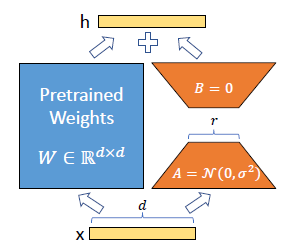
\includegraphics[scale=0.7]{Figures/Lora_brief.png}}
    \caption{The diagram of LoRA technique to reduce down trainable parameters for efficiency}
    \label{fig:Lora}
\end{figure}

\subsection{SFTTrainer}
Supervised Fine-Tuning Trainer, in short for SFTTrainer, is a trainer optimised for fine-tuning pre-trained models with smaller datasets to train\cite{Mudadla_2023}. It is mainly for supervised learning tasks\cite{Mudadla_2023}. It also trains faster and efficiently use memory while training as it is compatible with \textit{PEFT}\cite{Mudadla_2023}. These attributes are highly beneficial for this part of implementation as Llama2 will use significant amount of memory and will train slower than any models that is implemented in this project. The dataset that the project used is also small therefore using SFTTrainer instead of standard Trainer will be essential for training Llama2. The implementation of SFTTrainer is as shown in the listing(\ref{lst:SFTTrainer}).

\begin{lstlisting}[language=Python, caption=The code for SFTTrainer, label=lst:SFTTrainer]
    trainer = SFTTrainer(
        model=model,
        args=training_arguments,
        train_dataset=train_data,
        eval_dataset=val_data,
        peft_config=peft_config,
        dataset_text_field="text",
        tokenizer=tokenizer,
        max_seq_length=1024,
        packing=False,
        dataset_kwargs={
            "add_special_tokens": False,
            "append_concat_token": False,
        }
    )
\end{lstlisting}

\section{Testing Metrics}
After training the model, testing is needed to be done to see how the models perform after the training. Test dataset is used to test the model. There are two methods used to test the models, \textit{predict} and \textit{evaluate} functions from \textit{Trainer} class, and functions implemented from scratch. The \textit{predict} functions from \textit{Trainer} only provides the logits of the prediction outputs and metrics such as overall accuracy, f1-score and other metrics which are not of used for the analysis. For the \textit{evaluate} function from \textit{Trainer}, it outputs metrics only.

The \textit{predict} funtion created from scratch will output index of the labels instead of the logits. The \textit{evaluate} function will print out overall accuracy, accuracies for each labels, classification report which includes precision, recall, f1-score and support of each labels as well as the average, and confusion matrix. Those metrics are from \textit{sklearn.metrics} library. The code for both functions are listed below as listing(\ref{lst:predict_func}) and (\ref{lst:evaluate_func}) respectively.

\begin{lstlisting}[language=Python, caption=The code for predict function implemented, label=lst:predict_func]
    def predict(model, tokenizer):
    y_pred = []

    for i in tqdm(range(len(X_test))):

        prompt = X_test.iloc[i]["text"]
        pipe = pipeline(task="text-classification",
                        model=model,
                        tokenizer=tokenizer,
                       )
        result = pipe(prompt)
        answer = result[0]['label'].split("=")[-1]
        if "sadness" in answer:
            y_pred.append(0)
        elif "joy" in answer:
            y_pred.append(1)
        elif "love" in answer:
            y_pred.append(2)
        elif "anger" in answer:
            y_pred.append(3)
        elif "fear" in answer:
            y_pred.append(4)
        else:
            y_pred.append(5)

    return y_pred
\end{lstlisting}

\begin{lstlisting}[language=Python, caption=The code for evaluate function implemented, label=lst:evaluate_func]
def evaluate(y_true, y_pred):

    # Calculate accuracy
    accuracy = accuracy_score(y_true=y_true, y_pred=y_pred)
    print(f'Accuracy: {accuracy:.3f}')

    # Generate accuracy for each labels
    unique_labels = set(y_true)  # Get unique labels output: {0,1,2,3,4,5}

    for label in unique_labels:
        # will output a list of the index of one emotion at a time
        label_indices = [i for i in range(len(y_true))
                            if y_true[i] == label]
        # will output the list of one emotion
        label_y_true = [y_true[i] for i in label_indices]
        # label_y_true = [label for i in range(len(y_true))]
        # will output list of the predicted emotion in the same order as label_y_true
        label_y_pred = [y_pred[i] for i in label_indices]
        accuracy = accuracy_score(label_y_true, label_y_pred)
        print(f'Accuracy for label {label}: {accuracy:.3f}')

    # Generate classification report
    class_report = classification_report(y_true=y_true, y_pred=y_pred)
    print('\nClassification Report:')
    print(class_report)

    # Generate confusion matrix
    conf_matrix = confusion_matrix(y_true=y_true, y_pred=y_pred, labels=['sadness', 'joy', 'love', 'anger', 'fear', 'surprise'])
    print('\nConfusion Matrix:')
    print(conf_matrix)
\end{lstlisting}